\documentclass[a4paper,12pt]{article}
\usepackage{amsmath}
%\usepackage{polish}
\usepackage[polish]{babel}
\usepackage[utf8]{inputenc}
\usepackage[T1]{fontenc}
\usepackage{graphicx}
\usepackage{anysize}
\usepackage{enumerate}
\usepackage{times}
\usepackage{plain}
\usepackage{caption}
\usepackage{graphicx}
\usepackage{setspace}
\usepackage{multirow}
\usepackage{datetime}
\usepackage[outputdir=build]{minted}
\usepackage{xcolor}
\usepackage[colorlinks=true]{hyperref}
\usepackage[automake, acronyms, toc, nopostdot, nonumberlist]{glossaries}
\usepackage{indentfirst}
\hypersetup{
  colorlinks=true,
  linkcolor=blue,
  filecolor=magenta,
  urlcolor=cyan,
}
\urlstyle{same}
%\marginsize{left}{right}{top}{bottom}
\marginsize{2.5cm}{2.5cm}{2.5cm}{2.5cm}
\setlength{\parindent}{4em}
\setlength{\parskip}{1em}
\renewcommand{\baselinestretch}{2.0}

% listings with page breaking
\newenvironment{longlisting}{\captionsetup{type=listing}}{}

\definecolor{bg}{rgb}{0.95,0.95,0.95}
\setminted{
  fontfamily=txtt,
  fontsize=\footnotesize,
  samepage=false,
  style=xcode,
  breaklines,
  bgcolor=bg
}

% custom lexers for toml, ladr and spass
\newminted[tomlcode]{lexers/toml.py:TomlLexer -x}{}
\newmintinline[tomlcodeinline]{lexers/toml.py:TomlLexer -x}{}
\newmintedfile[tomlfile]{lexers/toml.py:TomlLexer -x}{}

% custom lexers for ladr, ladr and spass
\newminted[ladrcode]{lexers/ladr.py:LadrLexer -x}{}
\newmintinline[ladrcodeinline]{lexers/ladr.py:LadrLexer -x}{}
\newmintedfile[ladrfile]{lexers/ladr.py:LadrLexer -x}{}

% custom lexers for spass, ladr and spass
\newminted[spasscode]{lexers/spass.py:SpassLexer -x}{}
\newmintinline[spasscodeinline]{lexers/Spass.py:SpassLexer -x}{}
\newmintedfile[spassfile]{lexers/spass.py:SpassLexer -x}{}

\makeglossaries
\loadglsentries{glossaries}
\glsaddall

\begin{document}
\onehalfspacing
\begin{figure}[!htb]
  \centerline{
\includegraphics[scale=0.8]{images/agh_logo.jpg}}
\end{figure}

\begin{center}
  \Huge{Studio projektowe 1\\}
  \Large{Benchmark solverów prover9 oraz SPASS\\ \large \textit \today \\}
  \vspace{3cm}
  \Large{	Autorzy:\\
    Mateusz Grzeliński\\
    Przemysław Michałek\\
  }
  \large{Wydział Elektrotechniki, Automatyki, Informatyki i Elektroniki}

  \newpage
\end{center}

\tableofcontents
\newpage

\section{Streszczenie}

Celem projektu jest zbadanie wydajności automatyczych metod dowodzenia twierdzeń Prover9 oraz SPASS. Na początku zostaje wygenerowna formuła \gls{SAT}, która zostaje rozwiązana przez badane provery. Badany jest czas wykonania, rezultat (czy \gls{SAT} jest spełnialny), użycie pamięci RAM.
Generowana formuła \gls{SAT} jest modyfikowana ze względu na między innymi długość formuły, ilość zmiennych.

Provery traktowane są jako czarne skrzynki (blackbox), ich parametry są modyfikowane z poziomu linii komend.

\section{Benchmark}

Problem benchmarku w strategii blackbox sprowadza sie do wykonania podprogramu z odpowiednimi opcjami z poziomu linii komend.
Wejście oraz testy benchmarka ustawiane są poprzez plik konfiguracyjny, sekcja \ref{benchmarkUsage}.  Wejściem testu jest zbiór formuł \gls{SAT} zapisanych na dysku w formacie TPTP w postaci pliku tesktowego. Test polega na podaniu pliku TPTP do provera. W razie potrzeby nastąpi automatyczna konwersja do odpowiedniej składni za pomocą dostępnych translatorów.
Dla każdego provera dostępne są statystyki:

\begin{itemize}
  \item czas wykonania
  \item użycie pamięci RAM
  \item spełnialność formuły
\end{itemize}

\noindent
Więcej statystyk może zostać zebrany przez parser, który bada wyjście provera (sekcja \ref{parser}).
\newline
Zbadane zostaną statystyki proverów ze względu na następujące właściwości formuły SAT:

% more here:http://www.tptp.org/TPTP/TR/TPTPTR.shtml#ProblemGenerators
\begin{itemize}
  \item SAT type (CNF, FOF)
  \item number of clauses
    Clause is disjunction of a number of variables (negations may be present)
  \item number of atoms
  \item maximal clause size
  \item number of predicates
  \item number of functors
  \item number of variables
    variables assume values either 1 (true) or 0 (false)
  \item maximal term depth
\end{itemize}

For example, in expresion \mintinline{text}{(A v ¬B v C) ^ (B v D v E) ^ (D v F)} there are 3 clauses, 6 variables

\begin{figure}[H]
  \centering
  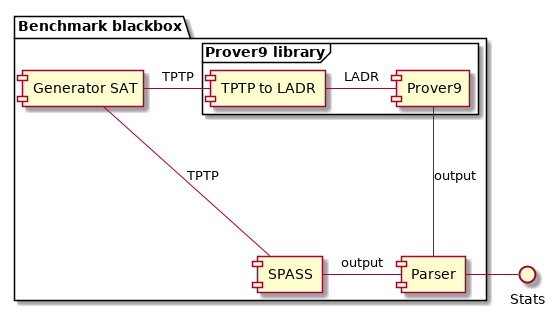
\includegraphics[scale=0.5]{benchmark/components.png}
  \caption{Diagram komponentów systemu benchmarka}
\end{figure}

\subsection{Prover9}

Prover9 jest to zautomatyzowane narzędzie udowadniające dla logiki pierwszego rzędu stworzone przez Williama McCune’a.

Prover9 dostępny jest jako plik wykonywalny, przyjmuje pliki w formacie \gls{LADR}. Dla uniwersalności zostanie zastosowany konwerter TPTP do LADR dostępny wraz z Proverem9 jako osobny plik wykonywalny. Ilość opcji dostępnych z lini komend jest minimanlna, jedyną ważną opcją z punktu widzenia benchmarka jest \mintinline{text}{-x - set(auto2).  (enhanced auto mode)}

\noindent
Oficjalna strona internetowa \url{https://www.cs.unm.edu/~mccune/mace4/}

\begin{longlisting}
  \caption{Przykład pliku wejściowego w składni LADR}
  \ladrfile{listings/prover9_example.in}
\end{longlisting}

\begin{longlisting}
  \caption{Przykład wyjścia Provera9}
  \inputminted{text}{listings/prover9_example.out}
\end{longlisting}

\subsubsection{TPTP to LADR}

W bibliotece \gls{LADR}, która jest załączona wraz ze źródłami Provera9, dostępny jest translator składni TPTP do LADR. Jest to plik wykonywalny. Na standardowe wejście przyjmuje TPTP, na standardowy wyjście podaje LADR.

Alternatywą do konwertera dostarczanego razem z prover9 jest program \mintinline{text}{tptp2X} dostarczanego przez TPTP.

\subsection{SPASS}

SPASS Theorem Prover jest narzędziem do automatycznego dowodzenia twierdzeń, należących do rachunku predykatów pierwszego rzędu.

SPASS nie korzysta z zewnętrznych bibliotek, dostępny jest jako plik wykonywalny. Akceptuje pliki w składni TPTP lub swojej własnej. SPASS udostępnia wiele opcji z poziomu lini komend. Z punktu widzenia benchmarka istotnymi są:

\begin{itemize}
  \item TODO
\end{itemize}

\noindent
Wszystkie opcje linii komend \url{https://webspass.spass-prover.org/help/options.html}
\noindent \newline
Oficjana strona internetowa \url{https://webspass.spass-prover.org/}

\begin{longlisting}
  \caption{Przykład pliku wejściowego w składni SPASS}
  \spassfile{listings/spass_example.in}
\end{longlisting}

\begin{longlisting}
  \caption{Przykład wyjścia SPASS}
  \inputminted{text}{listings/spass_example.out}
\end{longlisting}

\subsection{TPTP}

TPTP - \textit{ang. (Thousands of Problems for Theorem Provers)} - to biblioteka problemów wykorzystywanych do testowania systemów \gls{ATP}. Jednocześnie jest to nazwa formatu, w którym zapisywane są te testy. TPTP udostępnia te problemy na oficjalnej stronie intenetowej. Razem z TPTP istnieje TSTP (\textit{ang. Thousands of Solutions from Theorem Provers}) - biblioteka rozwiązań problemów.
Te problemy są sklasyfikowane przez domeny (3 literowe skróty), przykładowo LCL - Logic Calculi, COL - Combinatory Logic

W formacie TPTP można zapisywać \gls{TPI}, \gls{THF}, \gls{TFF}, \gls{FOF}, \gls{CNF}. Celem benchmarka jest badanie proverów logiku pierwszego rzędu, więc interesują nas \gls{CNF}, \gls{TFF}, \gls{FOF} (TFF/FOF with external clausifiers).

% from technical manual http://www.tptp.org/TPTP/TR/TPTPTR.shtml
\subsubsection{Wybrane elementy składni TPTP}

\begin{itemize}
  \item The syntax for atoms is that of Prolog: variables start with upper case letters, atoms and terms are written in prefix notation, uninterpreted predicates and functors either start with lower case and contain alphanumerics and underscore, or are in 'single quotes'.

  \item Each logical formula is wrapped in an annotated formula structure of the form  \newline \mintinline{text}{language(name,role,formula,source,[useful_info])}

    \begin{itemize}
      \item role gives the user semantics of the formula, one of
        \mintinline{text}{axiom},
        \mintinline{text}{hypothesis},
        \mintinline{text}{definition},
        \mintinline{text}{assumption},
        \mintinline{text}{lemma},
        \mintinline{text}{theorem},
        \mintinline{text}{corollary},
        \mintinline{text}{conjecture},
        \mintinline{text}{negated_conjecture},
        \mintinline{text}{plain},
        \mintinline{text}{type},
        and \mintinline{text}{unknown}.  Axiom-like formulae are those with the roles
        \mintinline{text}{axiom},
        \mintinline{text}{hypothesis},
        \mintinline{text}{definition},
        \mintinline{text}{assumption},
        \mintinline{text}{lemma},
        \mintinline{text}{theorem},
        and \mintinline{text}{corollary}. They are accepted, without proof, as a basis for proving conjectures in THF, TFF, and FOF problems. In CNF problems the axiom-like formulae are accepted as part of the set whose satisfiability has to be established. \mintinline{text}{conjecture} occur in only THF, TFF, and FOF problems, and are to all be proven from the axiom(-like) formulae. A problem is solved only when all conjectures are proven. TPTP problems never contain more than one conjecture. \mintinline{text}{negated_conjectures} are formed from negation of a \mintinline{text}{conjecture}, typically in FOF to CNF conversion.
      \item The \mintinline{text}{useful_info} field of an annotated formula is optional, and if it is not used then the \mintinline{text}{source} field becomes optional. The \mintinline{text}{source} field is used to record where the annotated formula came from, and is most commonly a file record or an inference record.
    \end{itemize}

  \item The language also supports interpreted predicates and functors. These come in two varieties: defined predicates and functors, whose interpretation is specified by the TPTP language, and system predicates and functors, whose interpretation is ATP system specific. The defined predicates recognized so far are \mintinline{text}{$true} and \mintinline{text}{$false} \mintinline{text}{=} and \mintinline{text}{!=} \mintinline{text}{$distinct} (only \gls{TFF} language) and  arithmetic predicates (only \gls{TFF} and \gls{THF}).
    Interpreted predicates and functors are syntactically distinct from uninterpreted ones - they are \mintinline{text}{=} and \mintinline{text}{!=}, or start with a \$, a '', or a digit. Non-variable symbols can be given a type globally, in the formula with role type. The defined types are \mintinline{text}{$o} - the Boolean type, \mintinline{text}{$i} - the type of individuals, \mintinline{text}{$real} - the type of reals, \mintinline{text}{$rat} - the type of rational, and \mintinline{text}{$int} - the type of integers. New types are introduced in formulae with the type role, based on \mintinline{text}{$tType} - the type of all types.

  \item The universal quantifier is \mintinline{text}{!}, the existential quantifier is \mintinline{text}{?}, and the lambda binder is \mintinline{text}{^}. Quantified formulae are written in the form \mintinline{text}{Quantifier [Variables] :  Formula}

  \item The binary connectives are infix \mintinline{text}{|} for disjunction, infix \mintinline{text}{&} for conjunction, infix \mintinline{text}{<=>} for equivalence, infix \mintinline{text}{=>} for implication, infix \mintinline{text}{<=} for reverse implication, infix \mintinline{text}{<~>} for non-equivalence (XOR), infix \mintinline{text}{~|} for negated disjunction (NOR), infix	\mintinline{text}{~&} for negated conjunction (NAND), infix \mintinline{text}{@} for application. The only unary connective is prefix \mintinline{text}{~} for negation

  \item  Arithmetic system are used in only the THF and TFF languages. This includes: 
    \mintinline{text}{$real} (real number)
    \mintinline{text}{$rat} (rational)
    \mintinline{text}{$to_int} (cast to int)
    \mintinline{text}{$to_rat}
    \mintinline{text}{$to_real}
    \mintinline{text}{$is_int}
    \mintinline{text}{$is_rat}
    \mintinline{text}{$is_real},
    unary operators:
    \mintinline{text}{$floor}
    \mintinline{text}{$round}
    \mintinline{text}{$ceiling}
    \mintinline{text}{$truncate},
    comparison of 2 numbers:
    \mintinline{text}{=}
    \mintinline{text}{$less}
    \mintinline{text}{$lesseq}
    \mintinline{text}{$greater}
    \mintinline{text}{$greatereq}
    \mintinline{text}{$uminus}
    \mintinline{text}{$sum}
    \mintinline{text}{$difference}
    \mintinline{text}{$product}
    \mintinline{text}{$quotient}
    \mintinline{text}{$quotient_e} (e for Euclidean quotient)
    \mintinline{text}{$quotient_t} (t for truncate)
    \mintinline{text}{$quotient_f} (f for floor)
    \mintinline{text}{$distinct}
    \mintinline{text}{$remainder_e}
    \mintinline{text}{$remainder_t}
    \mintinline{text}{$remainder_f}
\end{itemize}


\noindent
Oficjalna strona internetowa \url{http://www.tptp.org}
\newline
Pełny spis domen \url{http://www.tptp.org/cgi-bin/SeeTPTP?Category=Documents&File=THFSynopsis}
\newline
BNF składni TPTP \url{http://www.tptp.org/TPTP/SyntaxBNF.html}
\newline
Tutorial składni TPTP znajduje się pod linkiem \url{http://www.tptp.org/TPTP/TR/TPTPTR.shtml} Aby poznać jak zapisywana jest formuła, polecam przeczytać \textit{The Formulae Section}

\subsubsection{Narzędzia dodatkowe TPTP}

TPTP4X (napisane w c), TPTP2X (napisane w prologu) for reformatting, transforming, and generating TPTP problem files. Nie są używane w tym projekcie ale warto o nich wspomnieć, dostarczają wiele funkcjonalności.
Przykładowe możliwości:

\begin{itemize}
  \item konwertowanie \gls{FOF} do \gls{CNF}
  \item konwertowanie TPTP do składni prover9, dimacs, otter, dfg i więcej
  \item optymalizacja \gls{FOF}, \gls{CNF} za pomocą różnych algorytmów
  \item zmień porządek formuły \gls{CNF}
\end{itemize}

\subsection{Parser} \label{parser}

Zadaniem parsera jest wydobycie dodatkowych informacji statystycznych o przebiegu działana proverów, na podstawie ich wyjścia.
\newline
Każdy prover podaje inne dane na wyjściu, dostępne statystyki podane są w tabeli poniżej.
\newline
Statystyki zostaną podane w formacie json.

\begin{table}[ht]
  \centering
  \caption{Dostępne statystyki dla różnych proverów}
  \begin{tabular}{ |c|c|c| }
    \hline
    Prover & SPASS & Prover9 \\
    \hline
    SAT spełnialny & dostępny & dostępny \\
    \hline
    TODO & & \\
    \hline
  \end{tabular}
\end{table}

\subsection{Użycie i konfiguracja} \label{benchmarkUsage}

Ze względu na mnogośc opcji, większość opcji zawarta jest w pliku konfiguracyjnym \ref{configFile} w formacie \textit{toml}.

Najpierw definiowana jest lista wejść (\tomlcodeinline{testInput}). Wejście to zbiór plików, które można jednoznacznie zidentyfikować za pomocą nazwy (\tomlcodeinline{name}).
Następnie definiowana jest lista zestawów testowych (\tomlcodeinline{testSuite}). Zestaw testowy definiuje parametry wspólne dla kilku przypadków testowych (\tomlcodeinline{testCase}) np. ścieżka do pliku wykonywalnego. Każdy zestaw testowy posiada listę przypadków testowych. Każdy przypadek testowy definiuje w jakim formacie oczekuje wejście. Jeśli formaty są różne, konflikt jest rozwiązywany przy pomocy dostępnych translatorów. Opcje do testowania są definiowane jako lista. Plik wejściowy poże zosać podany przez standardowe wejście, przez opcję lini komend lub jako ostatni argument w komendzie.

\begin{minted}{bash}
testSuite.executable testSuite.options testSui.testCase.options
\end{minted}

\subsubsection{Wspierane funkconalności}

\begin{itemize}
  \item ścieżka do pliku wykonywalnego może być podana w pliku konfiguracyjnym, lub może być zawarta w zmiennyj środowiskowej \mintinline{text}{PATH} (ścieżka w pliku ma pierwszeństwo)
  \item definiowanie opcji linii komend do testowania pliku wykonywalnego
  \item definiowanie listy źródeł do testów. Źródłem do testów mogą być tylko pliki tesktowe
  \item definiowanie które wejścia mają byś przetestowane w przypadku testowym
    \begin{itemize}
      \item testuj tylko wymienione - opcja \tomlcodeinline{include_only},
      \item testuj wszystkich oprócz - opcja \tomlcodeinline{exclude},
      \item testuj wszystkie zdefiniowane wejścia - nie podając żadnej z opcji
    \end{itemize}
  \item pozycja nazwy pliku źródłowego może być ustawiona w następujący sposób
    \begin{itemize}
      \item podaj plik na standardowe wejście \tomlcodeinline{input_as_stdin}
      \item podaj plik jako ostatni argument \tomlcodeinline{input_as_last_argument}
      \item podaj plik jako argument po opcji \tomlcodeinline{input_after_option}
    \end{itemize}
  \item TODO: wyniki zapisywane są jako plik \textit{json} do katalogu wyściowego zdefiniowanego w pliku konfiguracyjnym.
\end{itemize}

\subsubsection{Ograniczenia}

\begin{itemize}
  \item podanie kilku plików wejściowych naraz dla jednej testownej komendy nie jest możliwe, np. \mintinline{text}{-o file1.p -o file2.p}
\end{itemize}

\begin{longlisting}
  \caption{Przykład pliku konfiguracyjnego benchmarka}
  \label{configFile}
  \tomlfile{benchmark/example_config.toml}
\end{longlisting}


\begin{longlisting}
  \caption{Przykładowe komendy testowe}
  \begin{tomlcode}
# ...
[[testSuites]]
executable="ls"
options=["-1"]
# ...

[[testSuites.testCases]]
options=[""]
# test cases:
# ls -1

[[testSuites.testCases]]
options=["", "-r -l"]
# test cases:
# ls -1
# ls -1 -r -l
  \end{tomlcode}
\end{longlisting}

\subsection{Diagramy}

\begin{figure}[H]
  \centering
  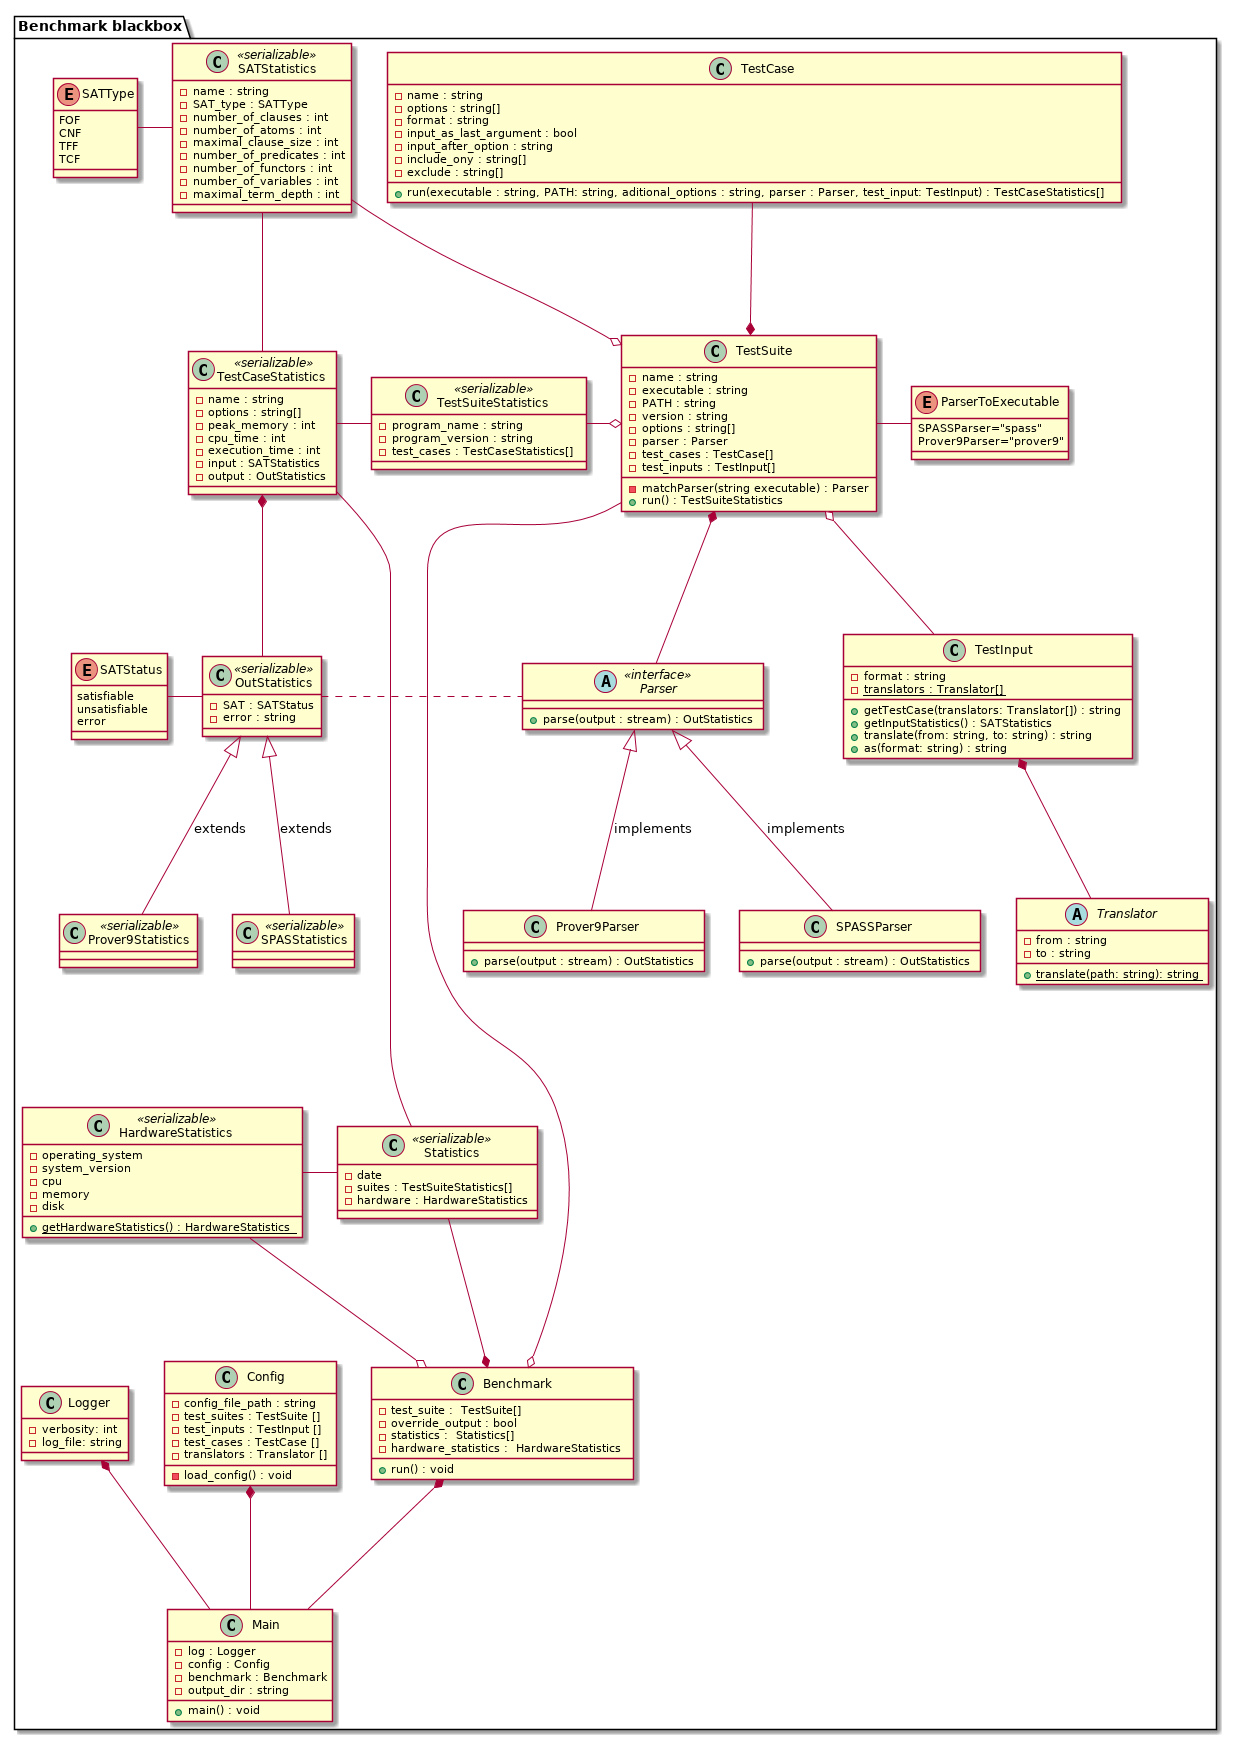
\includegraphics[width=0.9\textwidth]{benchmark/class_diagram.png}
  \caption{Diagram klas}
\end{figure}

\begin{figure}[H]
  \centering
  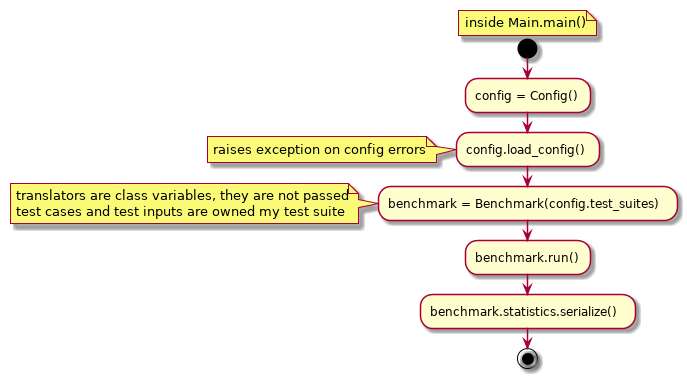
\includegraphics[width=\textwidth]{benchmark/activity_diagrams/main_run.png}
  \caption{Diagram aktywności}
\end{figure}

\begin{figure}[H]
  \centering
  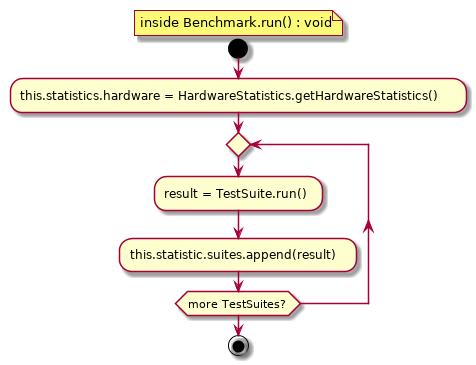
\includegraphics[width=0.8\textwidth]{benchmark/activity_diagrams/benchmark_run.png}
  \caption{Diagram aktywnośći}
\end{figure}

\begin{figure}[H]
  \centering
  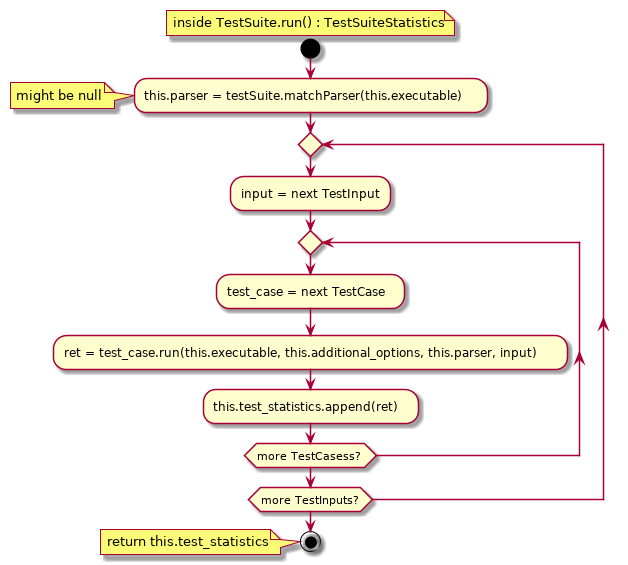
\includegraphics[width=\textwidth]{benchmark/activity_diagrams/test_suite_run.png}
  \caption{Diagram aktywnośći}
\end{figure}

\begin{figure}[H]
  \centering
  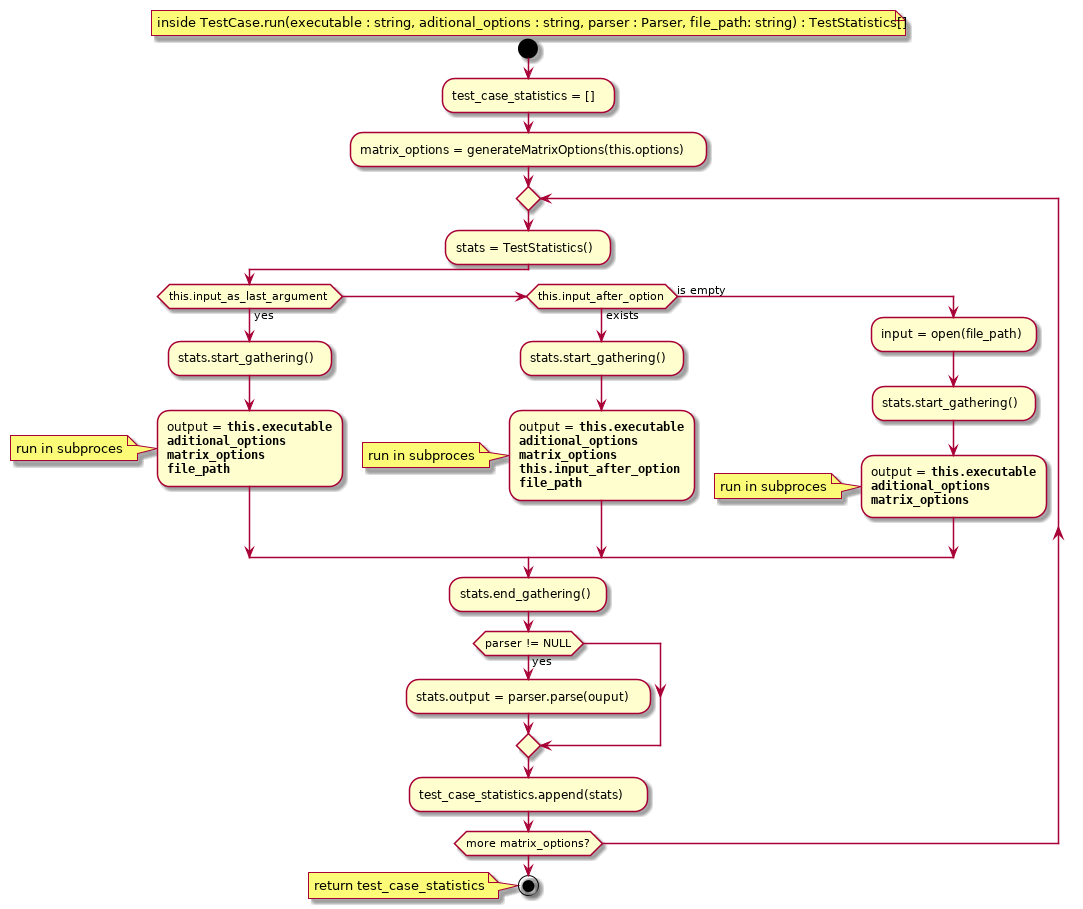
\includegraphics[width=\textwidth]{benchmark/activity_diagrams/test_case_run.png}
  \caption{Diagram aktywnośći}
\end{figure}

\section{Generator formuł logicznych} \label{LFG}

Generator formuł logicznych - \textit{ang. LFG - Logic formula generator} - losowy generator formuł SAT

\subsection{Wejście}

\begin{itemize}
  \item seed - opcjonalnie - umożliwia powtarzanie losowania
  \item typ generatora liczb losowych - opcjonalne, domyślnie \textit{uniform\_int\_distribution} \url{https://en.cppreference.com/w/cpp/named_req/RandomNumberDistribution} (TODO check if needed)
  \item ilość zmiennych - wymagane, integer
  \item ilość formuł - wymagane, integer
  \item generuj \gls{SAT} w formacie \gls{CNF}
    \begin{itemize}
      \item k-SAT z zadanym k
      \item Horn-SAT (TODO what is this exaclty?)
      \item NAE3SAT (TODO what is this exaclty?)
    \end{itemize}
  \item generuj \gls{SAT} spełnialny/niespełnialny/random - TODO czy jesteśmy w stanie wygenerować formułę, która będzie wiadomo że jest spełnialna lub nie? Można użyć do badania czy formuły poprawne są rozwiązywane szybciej.
\end{itemize}

\subsection{Wyjście}

\begin{itemize}
  \item string - SAT w formacie TPTP
\end{itemize}

\subsection{Algorytm generowania CNF}
\begin{itemize}
  \item Wypisz metadane jako komentarz (link do źródła, parametry wejściowe)
  \item TODO
\end{itemize}

\subsection{Algorytm generowania FOF}
\begin{itemize}
  \item Wypisz metadane jako komentarz (link do źródła, parametry wejściowe)
  \item TODO
\end{itemize}

\section{Wnioski}

Przykładowe wnioski

\subsection{Ilośc zmiennych}

\subsection{Stosunek ilości zmiennych do ilości formuł}

\subsection{Formuła w postaci CNF}

\printglossary[type=\acronymtype]
\printglossary

\end{document}
